\documentclass[11pt,a4paper]{article}

\usepackage[margin=2.2cm]{geometry}
\usepackage[T1]{fontenc}
\usepackage[utf8]{inputenc}
\usepackage{lmodern}
\usepackage{microtype}
\usepackage{graphicx}
\usepackage{fancyhdr}
\usepackage[hidelinks]{hyperref}

\setlength{\parindent}{0pt}
\setlength{\parskip}{6pt}
\pagestyle{fancy}
\fancyhf{}
\lhead{MLOps GBFS Bike-Sharing}
\rhead{Laporan Versioning Dataset}
\cfoot{\thepage}
\renewcommand{\headrulewidth}{0.4pt}
\renewcommand{\footrulewidth}{0pt}

\begin{document}

\begin{center}
{\LARGE\bfseries Laporan Versioning Dataset dengan DVC}\par
\vspace{4pt}
MLOps GBFS Bike-Sharing\par
20 Oktober 2026
\end{center}

\section*{Tujuan}
Membandingkan metadata dataset baseline dan versi baru menggunakan perintah
\texttt{dvc diff}. Perubahan isi dataset disimpan oleh DVC, sedangkan Git
melacak file pointer dan riwayat versinya.

\section*{Versi yang dibandingkan}
\begin{itemize}
  \item Baseline: commit \texttt{359df27} (\texttt{Track baseline processed data with DVC}).
  \item Versi baru: commit \texttt{4b1f91f} (\texttt{Add new GBFS data version}).
\end{itemize}

\section*{Bukti perintah \texttt{dvc diff}}
Berikut screenshot asli hasil perintah \texttt{dvc diff 359df27 4b1f91f --show-hash}:

\begin{center}
  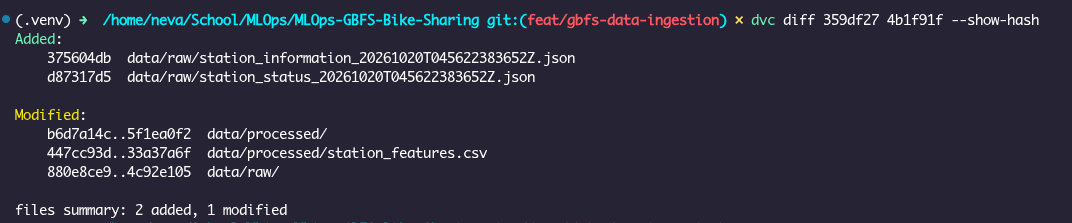
\includegraphics[width=\linewidth]{../dvc_screenshot.png}
\end{center}

\section*{Ringkasan perubahan}
Perbandingan menunjukkan dua file JSON GBFS baru ditambahkan ke
\texttt{data/raw/}. Hash direktori \texttt{data/raw/} dan
\texttt{data/processed/}, serta file \texttt{station\_features.csv}, berubah.
Ini menunjukkan data baru telah masuk dan perubahan dataset tercatat sebagai
versi DVC baru.

\section*{Penyimpanan dengan MinIO lokal}
File \texttt{compose.yaml} menyiapkan service MinIO dengan named volume.
Konfigurasi DVC remote \texttt{minio} menunjuk bucket \texttt{dvc-data} pada
endpoint \texttt{http://localhost:9000}. Kredensial akan disimpan secara lokal
di \texttt{.dvc/config.local}, bukan di Git.

\section*{Validasi dan status penyimpanan}
Perintah \texttt{dvc status} melaporkan bahwa data dan pipeline sudah sesuai
dengan metadata DVC. Konfigurasi MinIO sudah disiapkan, tetapi service belum
dijalankan dan \texttt{dvc push} belum dilakukan. Jadi, saat laporan ini dibuat,
object dataset masih tersimpan di local DVC cache.

\end{document}
